\documentclass[14pt,a4paper]{extreport}

\usepackage[utf8]{inputenc}
\usepackage[romanian]{babel}

% \renewcommand\familydefault{\sfdefault} % computer modern sans serif
\usepackage{fontspec}
\setmainfont{Times New Roman}


\linespread{1}

\usepackage{geometry}
 \geometry{
 left=20mm,
 right=10mm,
 top=20mm,
 bottom=20mm,
 % showframe
}

\usepackage{xcolor}
\definecolor{mygreen}{rgb}{0,0.6,0}
\definecolor{mygray}{rgb}{0.5,0.5,0.5}
\definecolor{mymauve}{rgb}{0.58,0,0.82}
\definecolor{darkgray}{rgb}{.4,.4,.4}
\definecolor{navy}{HTML}{000080}
\definecolor{purple}{rgb}{0.65, 0.12, 0.82}
\definecolor{codepurple}{rgb}{0.58,0,0.82}
\definecolor{backcolour}{rgb}{0.95,0.95,0.92}

% Please add the following required packages to your document preamble:
\usepackage{multirow}
\usepackage{array}

\usepackage{caption}
% \usepackage[singlelinecheck=false]{caption}

% \captionsetup[table]{name=Tabelul}

\usepackage{graphicx}
\graphicspath{ {./pictures/} }

\usepackage{amsmath} % for the equation* environment

\begin{document}

\begin{titlepage}
\begin{center}
	{\large{ Universitatea Tehnica a Moldovei \\}}
	{\large{ Facultatea Calculatoare, Informatică și Microelectronică \\}}
	{\large{ Departamentul Ingineria Software și Automatică \\}}
	\vspace{4cm}
	{\LARGE {\bf{ Raport }}}\\
	\vspace{1cm}
	{\large { Lucrarea de Laborator Nr.3 \\}}
	{\large { Metode și Modele de Calcul – 2 \\}}
	{\large { Tema: Probleme de Programare Liniara \\}}
\end{center}

\vspace{5cm}

\noindent{\large A efectuat:\hfill St. gr. TI-206} \\
\noindent{\large\null\hfill Pleșu Cătălin} \\
\noindent{\null} \\
\noindent{\large A verificat:\hfill Asist. Univ.} \\
\noindent{\large\null\hfill O. Buldumac} \\

\vspace{5cm}

\centering{\large{ Chișinău 2021 }}
\end{titlepage}


\clearpage
\subsection*{Scopul:\\}
Minimizarea și maximizarea problemelor de programare liniară.

\subsection*{Sarcina:}
\begin{enumerate}
	\item De formulat două probleme de programare liniară.
	\item PL minimizare - transport.
	\item PL maximizare - producție.
	\item De modelat matematic problemele.
	\item De optimizat problemele date prin metoda grafică.
	\item De realizat grafică în 2D a soluților pentru ambele
probleme: 
	\begin{itemize}
		\item dreptele formate de constrîngeri;
		\item regiunea admisibilă;
		\item coordonatele vârfurilor poligonului;
		\item este regiunea admisibilă mărginită sau nemărginită.
	\end{itemize}
	\item Problemele trebuie găsite sau formulate în așa fel ca regiunea admisibilă sa nu
fie vidă.
\end{enumerate}

\clearpage
\subsection*{PPL de Transport – Minimizare}
\paragraph{}
Chișinău și Bălți sunt centre de aprovizionare cu \textbf{produse alimentare} pentru centrele de desfacere
Ialoveni, Căușeni și Leova. 
Transportul se poate efectua de la oricare centru A\textsubscript{i} către oricare centru D\textsubscript{j}, existând un cost unitar C\textsubscript{ij}, al 
transportului unui bun de la centrul A\textsubscript{i} către centrul Dj. Astfel, costul total al 
transportului este proporţional cu cantitatea de bunuri transportate între sursă 
şi destinaţie. Datele problemei se află în Tabel ~\ref{tab:minimizare}. Unitățile ce țin de marfă sunt în camionae cu marfa respectivă.

\paragraph{}
\begin{table}[h]
\captionsetup{singlelinecheck = false, justification=raggedright}
\caption{Problema de minimizare a cheltuielilor pe transport}
\label{tab:minimizare} 
\begin{center}
\begin{tabular}{|l|l|l|l|l|}
\cline{2-4}
\multicolumn{1}{l|}{Ai\textbackslash{}Dj}&Ialoveni&Căușeni&Leova&\multicolumn{1}{l}{Disponibil}\\
\hline
Chișinău&\multicolumn{1}{l}{15}&\multicolumn{1}{l}{70}&100&100\\
\cline{1-1}\cline{5-5}
Bălți&\multicolumn{1}{l}{140}&\multicolumn{1}{l}{200}&200&200\\
\hline
\multicolumn{1}{l|}{Cererea}&150&75&75&\multicolumn{1}{l}{300}\\
\cline{2-4}
\end{tabular}
\end{center}
\end{table}


\paragraph{}
\begin{figure}[h]
\begin{center}
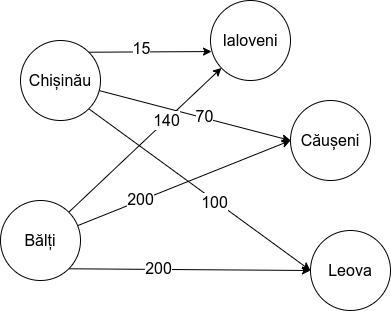
\includegraphics[width=12cm]{drumuri}
\caption{Reprezentarea grafica a costurilor de transport} 
\label{fig:drumuri}
\end{center}
\end{figure}

\paragraph{}
Dupa cum se vede din Figura ~\ref{fig:drumuri} și din tabelul
~\ref{tab:minimizare} problema data are 6 variaile și nu ar pute fi rezolvată
prin metoda grafică dacă nu am aduce-o mai întâi la 2 variablie.


\paragraph{}
\begin{table}[h]
\captionsetup{singlelinecheck = false, justification=raggedright}
\caption{Reducerea de la 6 variabile la 2}
\label{tab:reducere_min} 
\begin{center}
\begin{tabular}{|l|l|l|l|l|} 
\hline
Ai\textbackslash{}Dj& Ialoveni & Căușeni & Leova & Disponibil\\ 
\hline
\multirow{2}{*}{Chișinău} & 15 & 70& 100& \multirow{2}{*}{100}  \\
  & x  & y & 100 - x - y &  \\ 
\hline
\multirow{2}{*}{Bălți} & 140& 200  & 200& \multirow{2}{*}{200}  \\
  & 150 - x  & 75 - y  & x + y - 25  &  \\ 
\hline
Cererea & 150& 75& 75 & 300 \\
\hline
\end{tabular}
\end{center}
\end{table}


\paragraph{}
	Pentru a putea rezolva problema prin metoda grafică am notat prin x prima variabilă x\textsubscript{11} și y a doua variabilă x\textsubscript{12} astfel putem scrie funcția de calcul a prețului în felul următor:
\begin{equation*}
Z = 15x + 70y +10000 -100x -100y +21000 -140x + 15000 - 200y - 5000 + 200x + 200y
\end{equation*}

\paragraph{Modelul matematic}
Este necesar de gasit valorile nenegative ale variabilelor x și y pentru care funcția Z atinge valoarea minimă.

\begin{equation*}
Z = -25 x - 30 y + 41000 \rightarrow MIN
\end{equation*}

Restricții:

\begin{gather*}
	x + y \leq 100, \\
	x \leq 150, \\
	y \leq 75, \\
	x + y \geq 25, \\
	x \geq 0, \;
	y \geq 0.
\end{gather*}

\paragraph{}
Rezolvare. Construim poligonul convex al soluțiilor.

\begin{gather*}
	x + y = 100 \; (L1); \\
	x = 150 \; (L2); \\
	y = 75 \; (L3); \\
	x + y = 25 \; (L4); \\
	x = 0; \;
	y = 0.
\end{gather*}


\begin{figure}[h]
\begin{center}
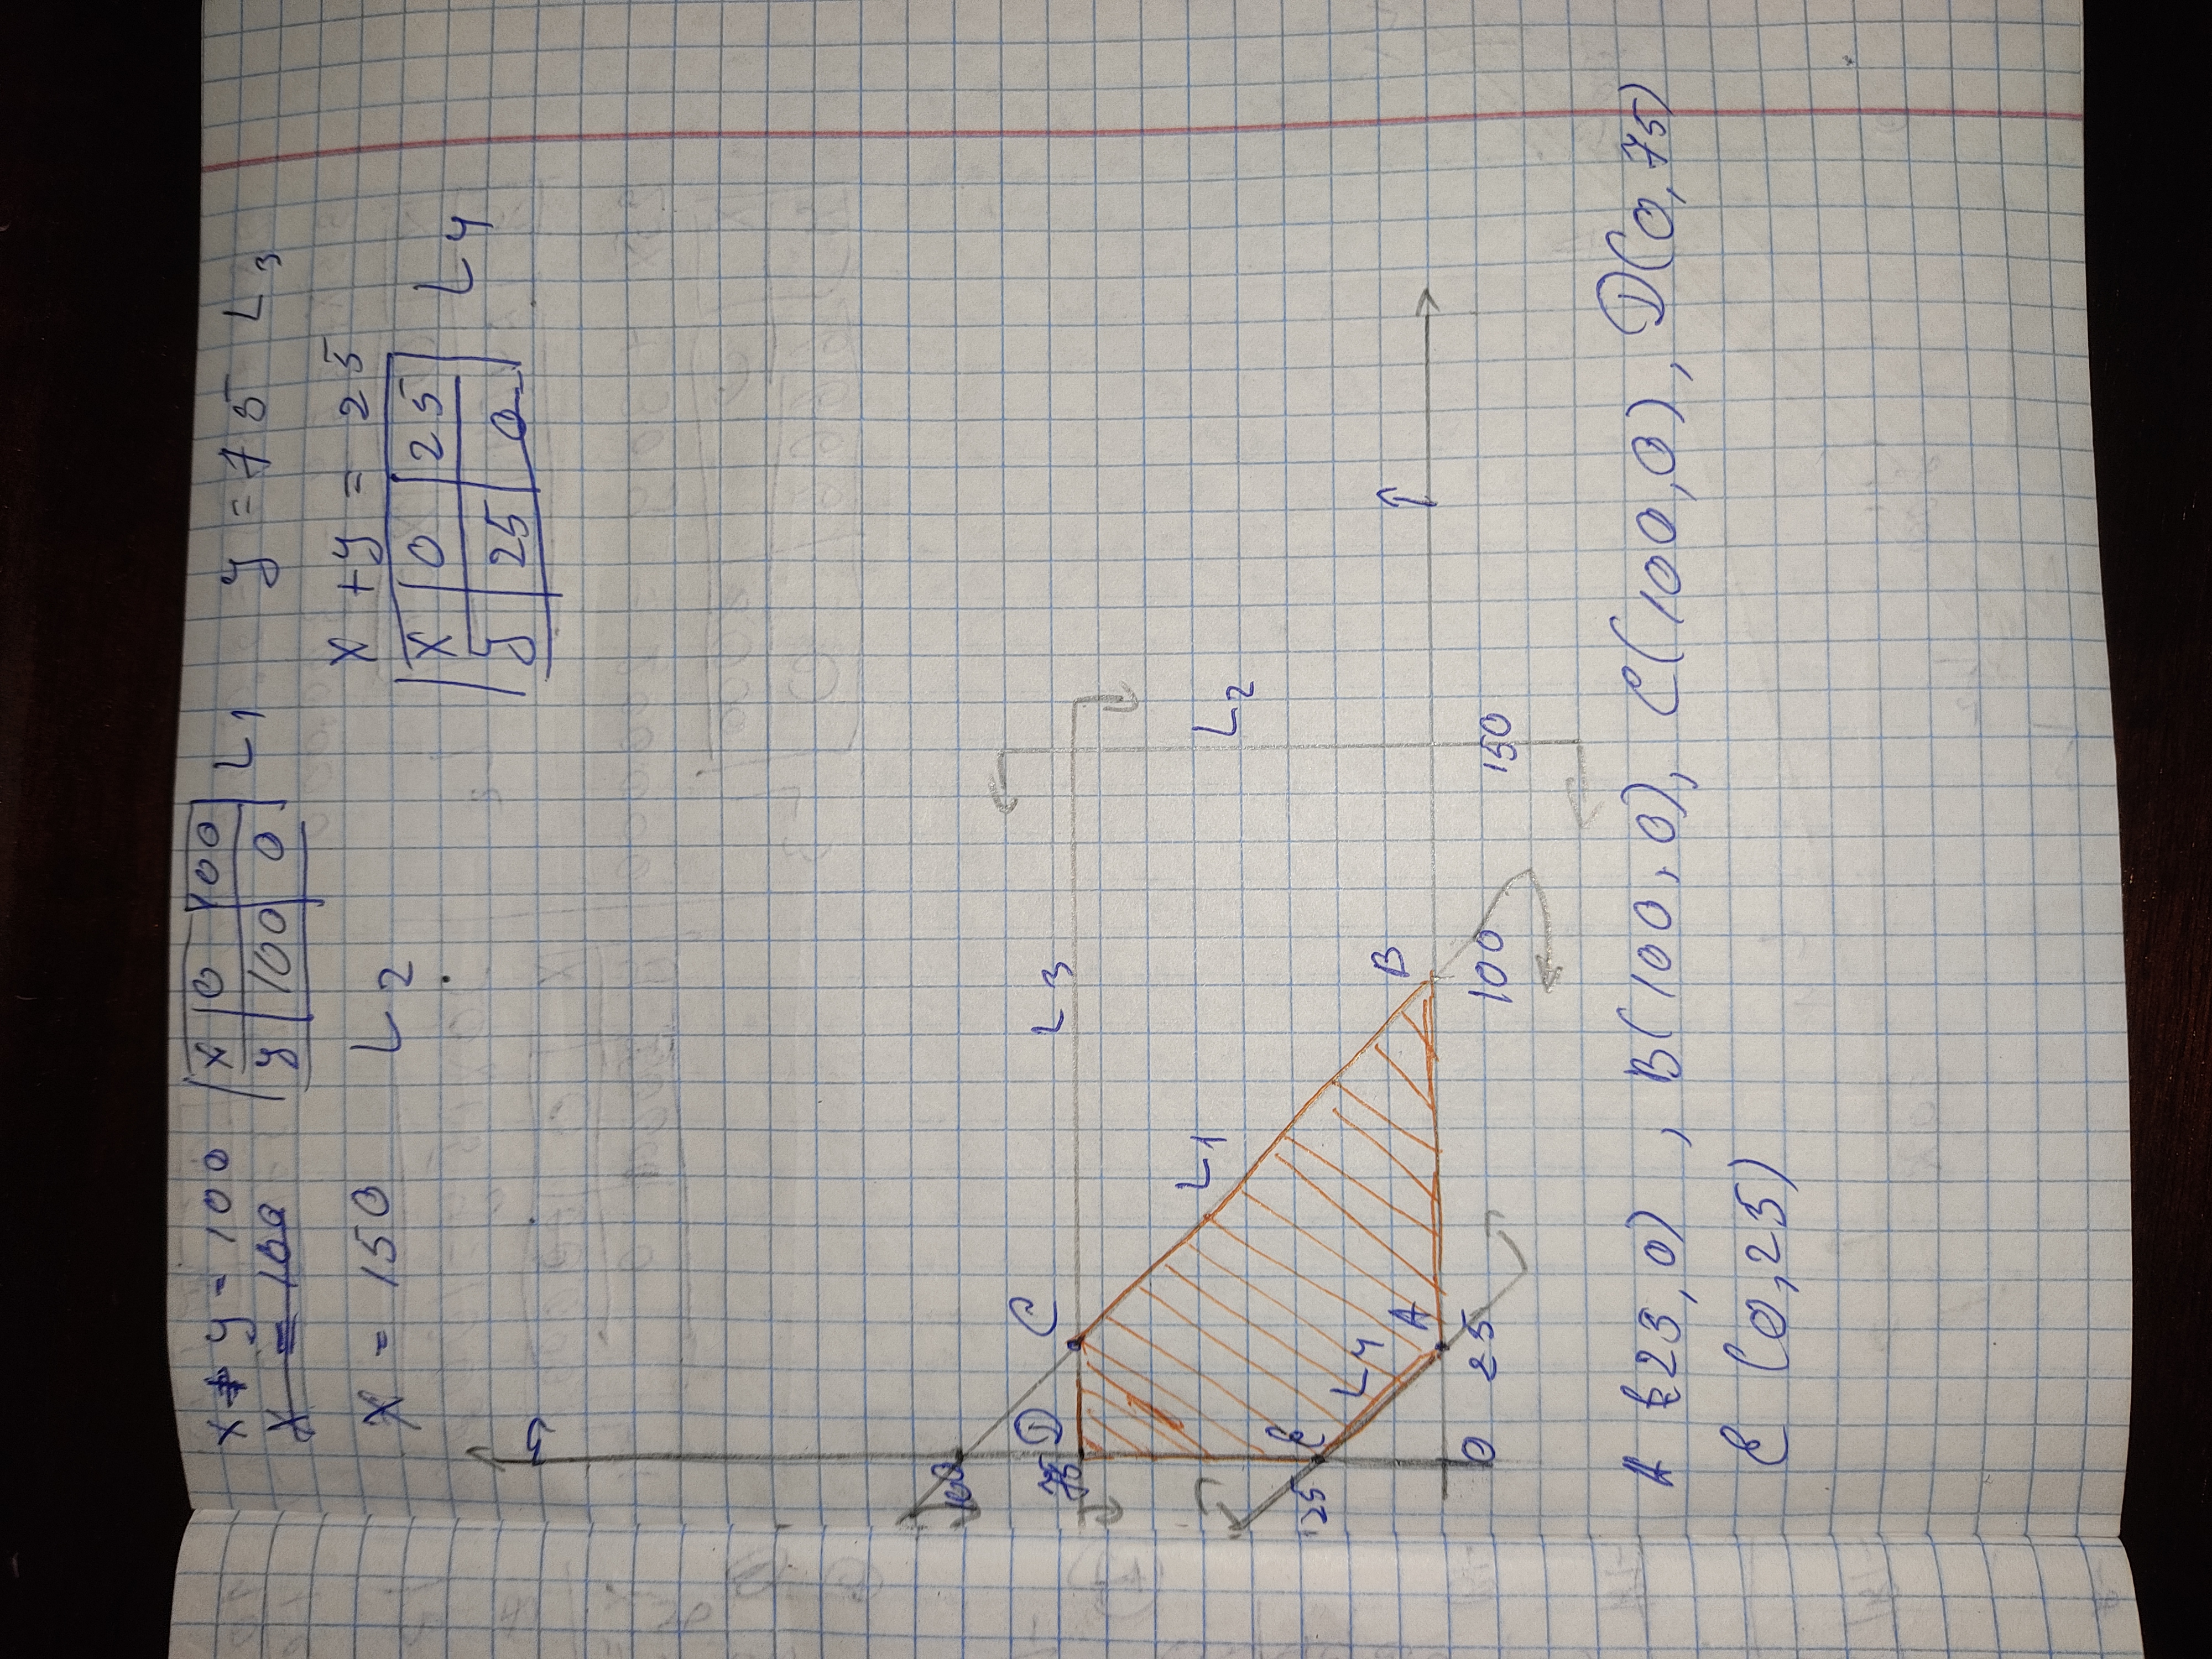
\includegraphics[width=15cm, angle=-90]{minimizare}
\caption{Poligonul convex solutiilor admisibile} 
\label{fig:minimizare}
\end{center}
\end{figure}

\paragraph{}

\paragraph{}
Poligonul convex are următoarele vârfuri: A(25,0), B(100,0), C(25,75), D(0,75), E(0,25)
\begin{gather*}
	Z(A) = -25 * 25 + -30 * 0 + 41000 = 40375 \\
	Z(B) = -25 * 100 + -30 * 0 + 41000 = 38500 \\
	Z(C) = -25 * 25 + -30 * 75 + 41000 = 38125 \\
	Z(D) = -25 * 0 + -30 * 75 + 41000 = 38750 \\
	Z(E) = -25 * 0 + -30 * 25 + 41000 = 40250 \\
\end{gather*}
După cum se observă vârful C este soluția optimă a problemei.

\paragraph{}
Rezultatul pentru problema de 2 variabile este x = 25; y = 75. Introducând valorile x și y în funcția liniară, obținem
\begin{equation*}
	Z\textsubscript{MIN} = -25 * 25 - 30 * 75 + 41000 = 38125 \\\end{equation*}
Acum putem substitui valorile x și y în tabelul inițial pentru a obține rezultatul final, valorile celor 6 variabile.

\paragraph{}
\begin{table}[h]
\captionsetup{singlelinecheck = false, justification=raggedright}
\caption{Introducea variabilelor x și y în tabel}
\label{tab:variabile_min} 
\begin{center}
\begin{tabular}{|l|l|l|l|l|} 
\hline
Ai\textbackslash{}Dj& Ialoveni & Căușeni & Leova & Disponibil\\ 
\hline
\multirow{4}{*}{Chișinău} & 15 & 70& 100 & 100 \\ 
\cline{2-5}
& x& y & 100 - x - y & \multirow{3}{*}{5625} \\
& 25 & 75& 0& \\
& 375 & 5250& 0& \\ 
\hline
\multirow{4}{*}{Bălți}& 140& 200 & 200 & 200 \\ 
\cline{2-5}
& 150 - x& 75 - y& x + y - 25& \multirow{3}{*}{32500}\\
& 125& 0& 75 & \\
& 17500& 0 & 15000 & \\ 
\hline
Cererea & 150& 75& 75& 300 \\
\hline
\end{tabular}
\end{center}
\end{table}

\paragraph{Răspuns }
În tabelul ~\ref{tab:variabile_min} am restabilit cele 6 variabile: 25, 75, 0, 125, 0, 75. Și le putem introduce în funcția Z:
\begin{gather*}
	Z= 
	c\textsubscript{11} * x\textsubscript{11} +  
	c\textsubscript{12} * x\textsubscript{12} +  
	c\textsubscript{13} * x\textsubscript{13} +  
	c\textsubscript{21} * x\textsubscript{21} +  
	c\textsubscript{22} * x\textsubscript{22} +  
	c\textsubscript{33} * x\textsubscript{33}  \rightarrow MIN  \\
Z\textsubscript{MIN} = 375 + 5250 + 0 + 17500 + 0 + 15000 = \\
= 5625 + 32500 = 38125
\end{gather*}


\clearpage
\subsection*{PPL de Productie – Maximizare}
\paragraph{}
O fabrică produce două tipuri de pițe congelate, pentru producerea acestor
produse se în calitate de materie primă se folosește aluat, salam, cașcaval și
măsline.Rezerva de materie primă, cantitatea de unități de materie primă
necesara pentru fabricarea unei unități de produs și mărimea venitului obținut
în urma realizării unei unități de produs sunt date in Tabel
~\ref{tab:maximizare}. Este necesar de alcătuit un plan de producție astfel
încât la realizarea ei să obținem venitul maximal.


\paragraph{}
\begin{table}[h]
\centering
\captionsetup{singlelinecheck = false, justification=raggedright}
\caption{Problema de maximizare a venitului}
\label{tab:maximizare}
\begin{center}
\begin{tabular}{|c|c|c|c|}
\hline
	\multirow{2}{3cm}{Tipuri de materie primă} & \multirow{2}{3cm}{Rezerva de materie primă} & \multicolumn{2}{>\centering m{10cm}|}{Cantitatea de materie primă necesară pentru fabricarea unei unități de produs}\\ 
\cline{3-4}
	&& \multicolumn{1}{>\centering m{5cm}|}{Diavola} & \multicolumn{1}{>\centering m{5cm}|}{Atomica}\\ 
\hline
Aluat&2000000&280 &350 \\
Salam&300000&35 &55 \\
Cașcaval&200000&25 &30 \\ 
Măsline&100000&20 &5 \\ 
\hline 
	\multicolumn{2}{|>\centering m{6cm}|}{Venitul de la realizarea unei unități de produs} & 45 & 50\\
\hline
\end{tabular}
\end{center}
\end{table}

\paragraph{Modelul matematic}
Este necesar de gasit valorile nenegative ale variabilelor x și y pentru care funcția Z atinge valoarea maximă.
\begin{gather*}
	Z = 45x + 50y \rightarrow MAX
\end{gather*}
Restricțiile:
\begin{gather*}
	280x + 350y \leq 2000000, \\
	35 x + 55 y \leq 300000, \\
	25 x + 30 y \leq 200000, \\
	20 x + 5 y\leq 100000, \\
	x \geq 0, \; y \geq 0.
\end{gather*}
Rezolvare. Construim tronsonul soluțiilor.
\begin{gather*}
	280x + 350y = 2000000 \; (L1);\\
	35 x + 55 y = 300000 \; (L2); \\
	25 x + 30 y = 200000 \; (L3); \\
	20 x + 5 y= 100000 \; (L4); \\
	x = 0; \; y = 0.
\end{gather*}

\begin{figure}[h]
\begin{center}
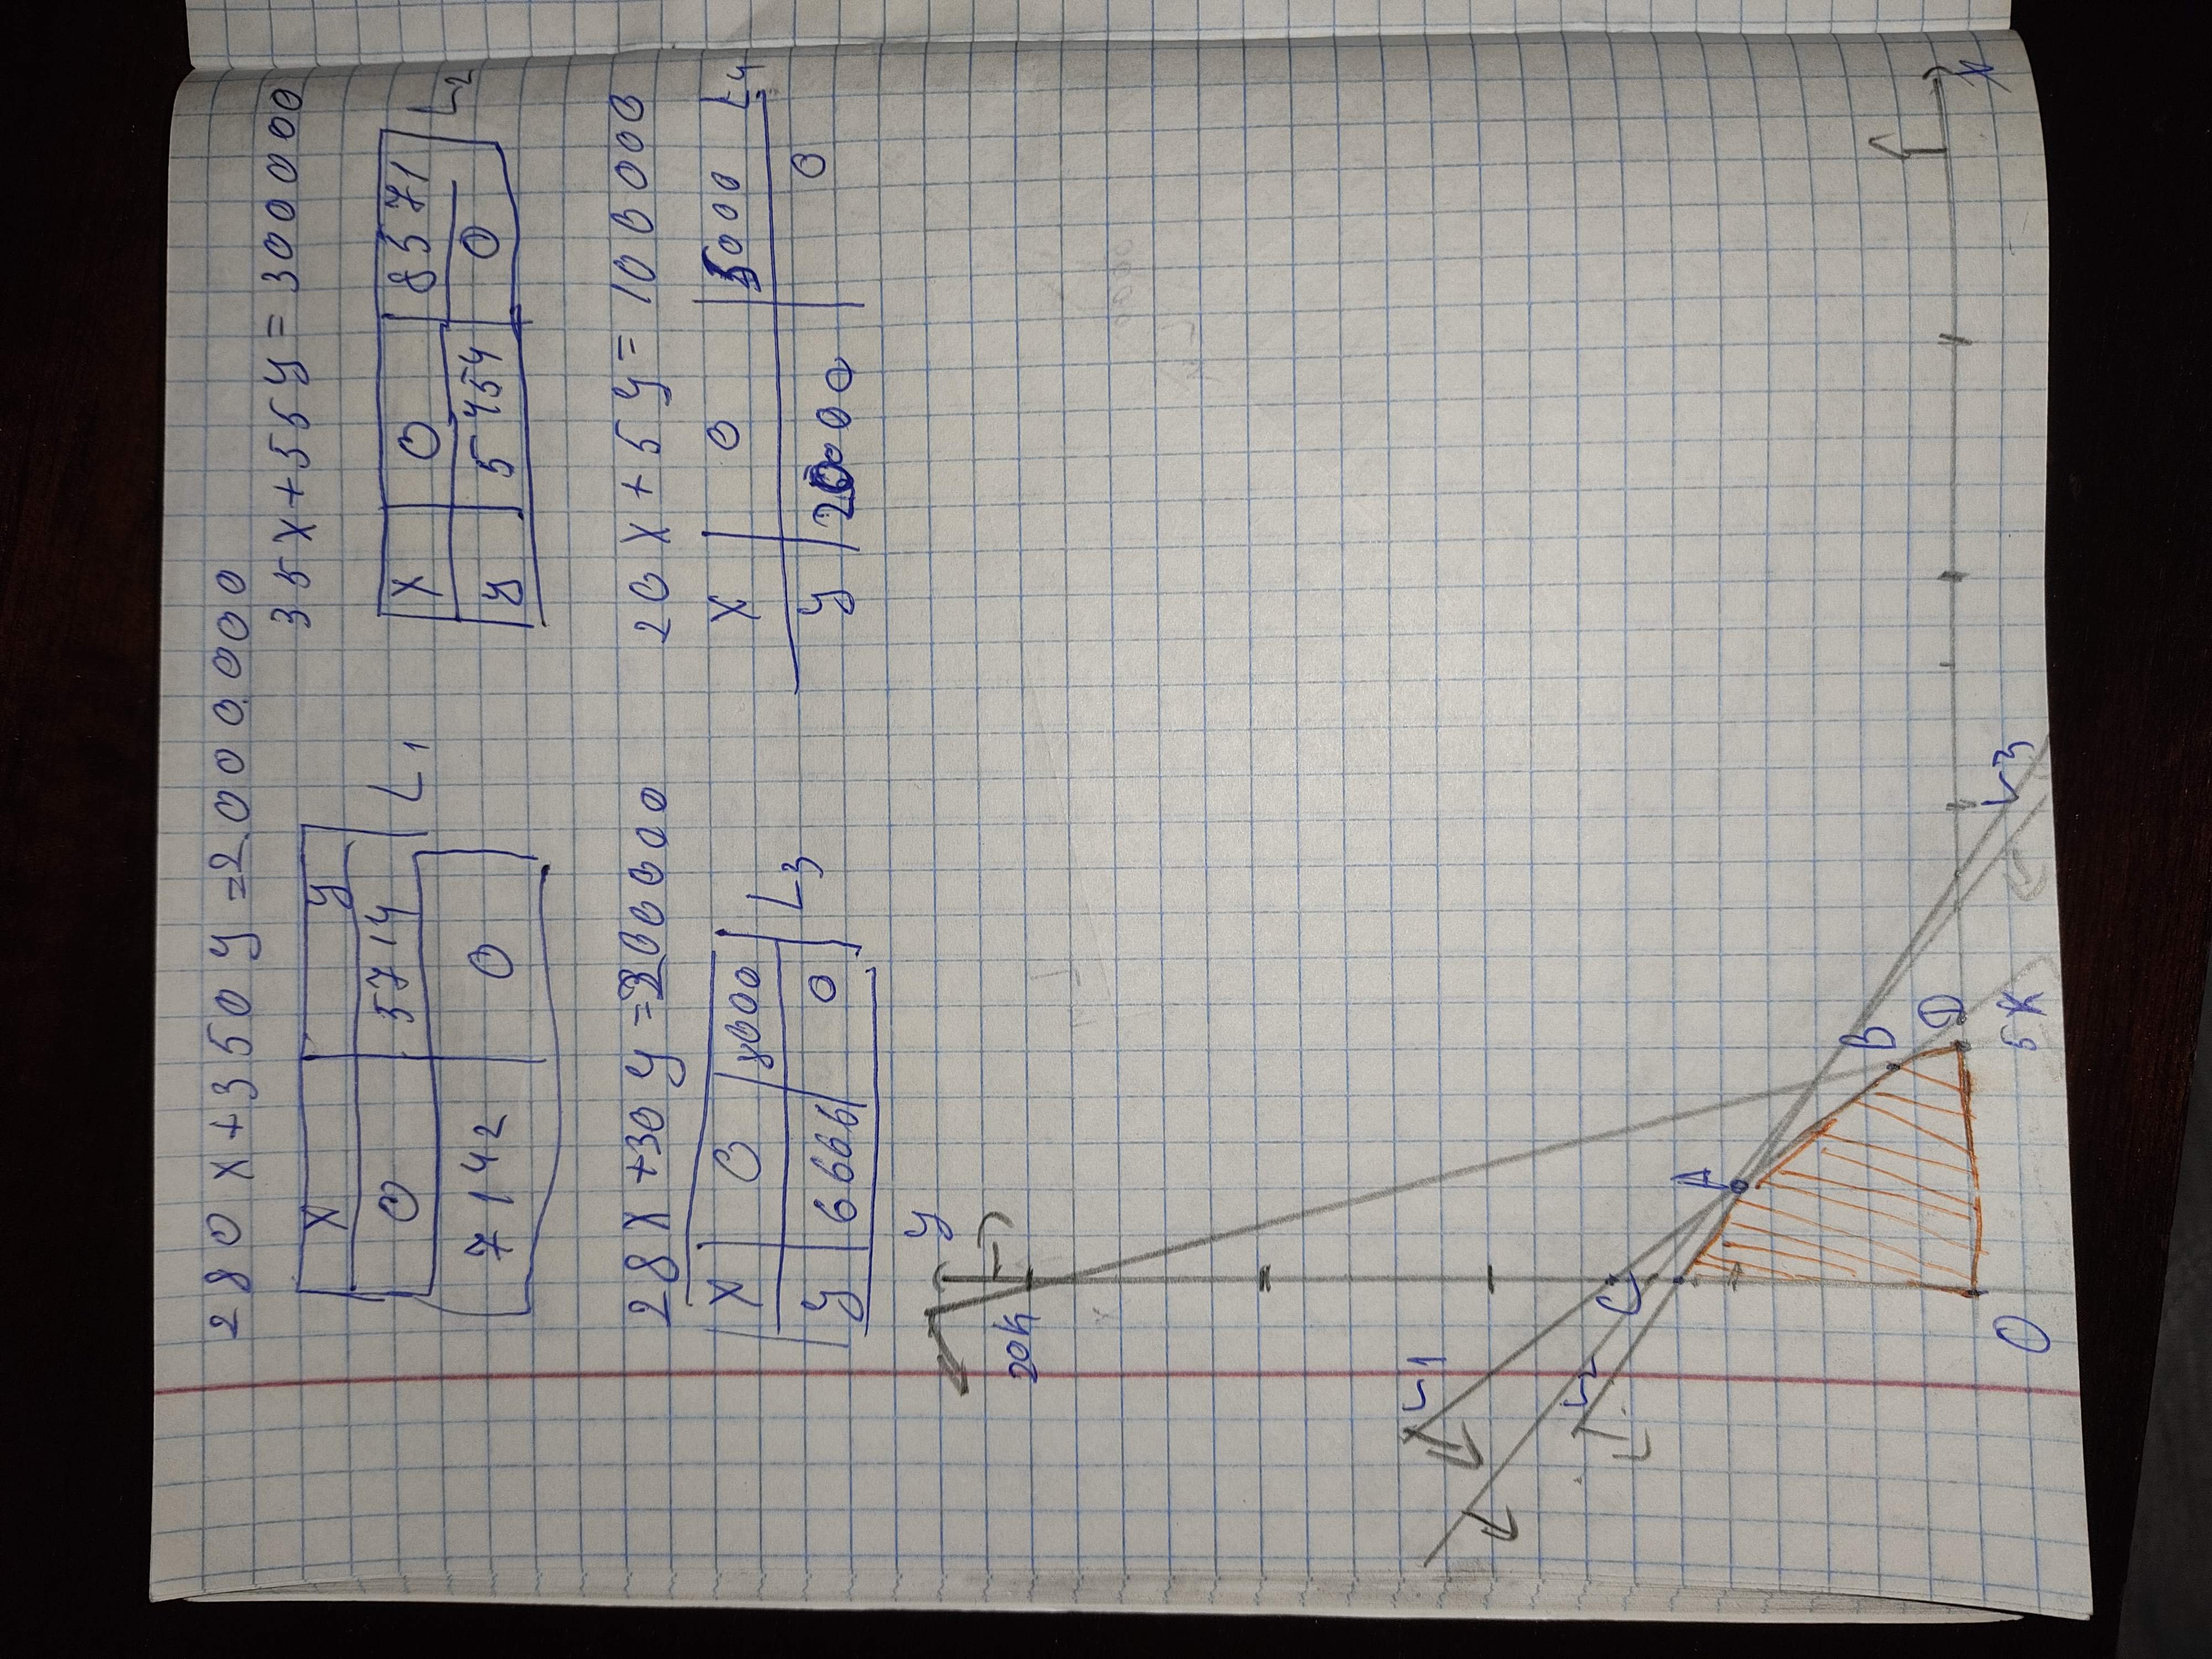
\includegraphics[width=15cm,angle=-90]{maximizare}
\caption{Tronsonul solutiilor admisibile} 
\label{fig:maximizare}
\end{center}
\end{figure}


\paragraph{}
	După cum se vede în Figura ~\ref{fig:maximizare} tronsonul data are 5 vârfuri iar în urma deplasării paralele a dreptei ce corespunde \( 45x + 50y = 0 \) pe vectorul N = (45; 50)\textsuperscript{T}.


\paragraph{}
Tronsonul are următoarele vârfuri: A=(1588,4444), B=(4464,2142), C=(0,5454), \\
D=(5000,0), O=(0,0).
\\
Conform metodei grafice în punctul B profitul este maxim.
\newline
\begin{gather*}
	Z(B) = 45 * 4464 + 50 * 2142 = 307980 \\
	Z(A) = 45 * 1588 + 50 * 4444 = 293666 \\
	Z(C) = 45 * 0 + 50 * 5454 = 272700 \\
	Z(D) = 45 * 5000 + 50 * 0 = 225000 \\
	Z(O) = 0
\end{gather*}


\paragraph{Răspuns }
rezultatul aproximativ este x = 4464; y = 2142. Introducând valorile x și y în funcția liniară, obținem
\begin{equation*}
	Z\textsubscript{MAX}= 45 * 4464 + 50 * 2142 = 307980
\end{equation*}



\clearpage
\paragraph{\large Concluzii:}\mbox{}\\

\subparagraph{}{
Am formulat două probleme de programare liniară una de transport și una de producție, am încercat ca datele din aceste probleme să fie cât mai realiste și m-am asigurat că regiunea admisibilă nu este vidă.
}

\subparagraph{}{
Am utilizat metoda grafică pentru a rezolva o problema de programare liniară de transport și o problemă de producție. Problema de transport a fost puțin mai dificilă fiind că inițial avea șase variabile.
}


\subparagraph{}{
Uitândune mai bine la regiunile admisibile putem observa ca pentru problema de transport regiunea admisibilă este un poligon convex, iar in cazul în care poligonul nu ar fi convex problema nu ar putea fi rezolvata, pentru problema de transport regiunea admisibilă conturează un tronson.
Pentru ambele probleme obținem regiunea admisibilă mărginită.
Rezultatele acestor probleme sunt unice, soluții mai bune fiind imposibil de găsit.
}

\subparagraph{}{
O problemă care ar fi putut apărea în urma rezolvării acestor probleme este obținerea unor valori cu zecimale pentru variabile fiind că pare specific că la producție so produc unități întregi iar la transport nu este garantat că tranportul unei cantități înjumătățite ar reduce prețul de transport. 
}

\subparagraph{}{
	\LaTeX
}


\end{document}
